    
\chapter{Kanji 漢字}

\begin{center}
\begin{Large}
第6課: Kanji 漢字: An Introduction 
\end{Large}
\end{center}
 
\par{  \emph{Kanji } ${\overset{\textnormal{かんじ}}{\text{漢字}}}$ are Chinese characters used in Japanese writing. Japanese is not a part of the same language family as Chinese, but thousands of words have been borrowed from Chinese to make \emph{Kanji }漢字 a fundamental aspect of Japanese culture. When \emph{Kanji } 漢字 are used to write a word, the y may provide meaning, sound, or both. Each character may have multiple meanings and readings, which are then chosen on a case-by-case basis. }

\par{ \emph{Kanji } 漢字 are primarily used to write words of Chinese origin. However, they are also important in writing the stems of verbs and adjectives and much more. Because there are at least 3,000 characters that are commonly used in Japanese today, it's not possible to learn them all in one go. However, this lesson will help you become familiar with the system as a wh ole so that learning them may be easier. }

\par{\textbf{Linguistic Note }: Japanese has received major influence from Chinese, but it is in its own language family called the Japonic language family. Japanese is related to other Japanese languages spoken in Okinawa. }

\par{\textbf{Notation Note }: Pitch contours are included in this lesson. High pitch morae are marked in bold and pitch falls are denoted by ↓. }
      
\section{ON \& KUN Readings}
 
\par{ There are two broad kinds of readings that \emph{Kanji } 漢字 may have: ON and KUN. ON readings are pronunciations that were borrowed into Japanese from various stage of Chinese over several centuries. KUN readings, on the other hand, come from native vocabulary with some semantic association with the \emph{Kanji } 漢字 in question. Consequently, most characters have more than one reading of each kind . Despite how complex all this may seem, there are patterns that you can utilize to make things easier. }

\par{\textbf{Spelling Note }: In the charts below, ON readings are rendered in \emph{Katakana }カタカナ and KUN readings are rendered in \emph{Hiragana }ひらがな. In reality, readings of words are normally usually given in \emph{Hiragana }ひらがな unless the phrase is a loan-word. }

\begin{center}
 \textbf{オン READINGS }
\end{center}

\par{ Almost all phrases composed of ON readings ( \emph{on'yomi } ${\overset{\textnormal{}}{\text{音}}}$ ${\overset{\textnormal{}}{\text{読}}}$ み) are Chinese in origin. All \emph{Kanji }漢字 that were made in China have \textbf{one or more }ON readings \textbf{with one or more meanings }. Even some \emph{Kanji } 漢字 that were made in Japan have ON readings. \hfill\break
\hfill\break
 \emph{Kanji }漢字 were borrowed from China in several waves from various time periods and locales in China, and in each wave, new characters as well as new readings of previously introduced characters were brought to Japan. }

\par{ ON readings are frequently used in \textbf{phrases made up of two or more \emph{Kanji }}漢字 . However, they can also be seen in single-character phrases, especially when the phrase has no native equivalent. Because etymology is not a source of information readily ascertainable right off the bat, it is always best to learn the readings of phrases on a case-by-case basis. }

\begin{ltabulary}{|P|P|P|P|P|P|P|P|}
\hline 

 \emph{Kanji }& \emph{Kana }& \emph{Rōmaji }& Meaning &  \emph{Kanji }& \emph{Kana }& \emph{Rōmaji }& Meaning \\ \cline{1-8}

知識 &  \textbf{チ }シキ &  \emph{Chishiki }& Knowledge & 天 &  \textbf{テ }ン &  \emph{Ten }& Heaven \\ \cline{1-8}

円 &  \textbf{エ }ン &  \emph{En }& Yen & 評価 &  \textbf{ヒョ }ウカ &  \emph{Hyōka }& Evaluation \\ \cline{1-8}

理由 & リ \textbf{ユウ }&  \emph{Riyū }& Reason & 工場 & コ \textbf{ウジョ }ウ &  \emph{Kōjō }& Factory \hfill\break
\\ \cline{1-8}

知事 &  \textbf{チ }ジ &  \emph{Chiji }& Governor & 死 &  \textbf{シ }↓ &  \emph{Shi }& Death \\ \cline{1-8}

\end{ltabulary}

\par{ \textbf{くん READINGS }}

\par{${\overset{\textnormal{}}{\text{KUN readings (訓読み)}}}$ are generally \textbf{native }words applied to \emph{Kanji }漢字 . 北 means north. The Japanese word for north is \emph{kita }きた, and in words from Chinese its ON reading \emph{hoku }ホク is used. \emph{Kanji }漢字 may have one or more KUN readings. They are commonly used in isolation unlike ON readings, but many are used in conjugations with \emph{Hiragana }ひらがな following. }

\begin{ltabulary}{|P|P|P|P|P|P|P|P|}
\hline 

 \emph{Kanji }& \emph{Kana }& \emph{Rōmaji }& Meaning &  \emph{Kanji }& \emph{Kana }& \emph{Rōmaji }& Meaning \\ \cline{1-8}

雨 &  \textbf{あ }め &  \emph{Ame }& Rain & 雨雲 & あ \textbf{まぐ }も &  \emph{Amagumo }& Rain cloud \\ \cline{1-8}

日傘 & ひ \textbf{が }さ &  \emph{Higasa }& Parasol & 日 & ひ &  \emph{\textbf{Hi }↓ }& Day \\ \cline{1-8}

思い & お \textbf{も }い &  \emph{Omoi }& Thought & 歌う & う \textbf{たう }&  \emph{Utau }& To sing \\ \cline{1-8}

小山 & こ \textbf{やま }&  \emph{Koyama }& Hillock & 高い & た \textbf{か }い &  \emph{Takai }& High \\ \cline{1-8}

\end{ltabulary}

\begin{center}
ON-KUN \& KUN-ON COMPOUNDS  
\end{center}

\par{ At times ON and KUN readings are used \emph{together }to make a compound. These readings are called \emph{Jūbako }readings ( \emph{j }\emph{ūbakoyomi }${\overset{\textnormal{}}{\text{重箱読}}}$ み) and \emph{Yutō }readings ( \emph{y }\emph{utōyomi }${\overset{\textnormal{}}{\text{湯桶読}}}$ み) respectively. \emph{Jūbako }ジュウばこ and \emph{Yutō }ゆトウ happen to be examples of the phenomena they represent. }

\begin{ltabulary}{|P|P|P|P|P|P|P|P|}
\hline 

 \emph{Kanji }& \emph{Kana }& \emph{Rōmaji }& Meaning &  \emph{Kanji }& \emph{Kana }& \emph{Rōmaji }& Meaning \\ \cline{1-8}

場所 & ば \textbf{ショ }&  \emph{Basho }& Place & 路肩 & ロ \textbf{かた }&  \emph{Rokata }& Road shoulder \\ \cline{1-8}

身分 &  \textbf{み }ブン &  \emph{Mibun }& Position; status & 台所 & ダ \textbf{イどころ }&  \emph{Daidokoro }& Kitchen \\ \cline{1-8}

消印 & け \textbf{しイン }&  \emph{Keshi'in }& Postmark & 見本 & み \textbf{ホン }&  \emph{Mihon }& Sample \\ \cline{1-8}

\end{ltabulary}

\par{\textbf{Practice }: }

\par{ Classify the following words by reading: ON, KUN, \emph{Jūbako }, or \emph{Yutō }. As you have only been introduced to \emph{Kanji }漢字, use a dictionary resource like jisho.org to look up the readings of the words and of the individual characters. As you do this, if you find any peculiar things, take note of them as those notes may be helpful to you. }

\par{1. 美しい  \hfill\break
2. 花  \hfill\break
3. 新聞  \hfill\break
4. 番組  \hfill\break
5. 手帳  }

\par{\textbf{Exercises }: }

\par{1. \emph{Kanji } 漢字 are typically written top-down and left to right. This is largely simplified, but it can prevent frivolous errors. Use a dictionary resource like jisho.org to look up the following \emph{Kanji }漢字 . }

\par{生  雨  長  金  風  中  円  魚  日  刀  土 小  上  山  女  男  子  海  耳 }

\par{2. Write out each \emph{Kanji }漢字 \emph{ }above 10 times. }

\par{3. Write out the readings, meanings, and examples on another sheet of paper. }
\textbf{Spelling Note }: \emph{オン readings are in カタカナ; くん readings are in ひらがな. In reality readings are normally only given in ひらがな unless the word is a loan. }\hfill\break
      
\section{Radicals 部首(ぶしゅ)}
 
\par{ Radicals are the building blocks of \emph{Kanji }漢字 . All \emph{Kanji }漢字 \emph{ }are made up of one or more of them. There are 214 radicals that exist in Japanese, and these are all neatly organized by stroke count below: }
 
\begin{figure}[h]
\centering

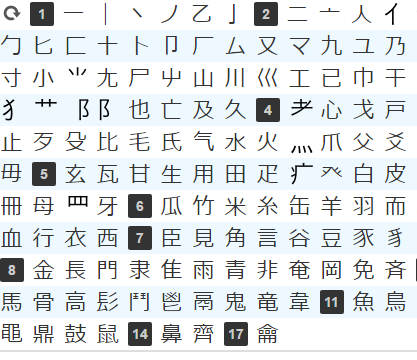
\includegraphics[width=0.9\textwidth]{figs/第01章/第6課:_kanjiintro_fig/Radicals_2.png}

\end{figure}

\par{\textbf{Resource\slash Citation Note }: Image taken from www.jisho.org, an amazing online dictionary perfect for researching what you want to know about \emph{Kanji }漢字 . }

\par{ \emph{Kanji } 漢字 with the \textbf{same radical }usually have \textbf{similar meaning }. For example, the \emph{Kanji }語, 訳, 訓, and 許 all have the radical for speech, which is 言, and they all have meanings related to speech. Sometimes, radicals are used for phonetic purposes. Therefore, \emph{Kanji } 漢字 with the \textbf{same phonetic }often have \textbf{similar ON readings }. The \emph{ }characters  時, 持, and 侍 all have the ON reading \emph{ji }ジ because the phonetic component 寺's ON reading is \emph{ji }ジ. There are exceptions to this method of guessing an ON reading, though. For example, 待 and 特 have the readings of \emph{tai }タイ and \emph{toku }トク.  Phonetics themselves may not always play a semantic role and don't help with KUN readings. }
 
\par{ Radicals do have names. However, it isn't essential for you to know what the names of the building blocks are. It is beneficial, though, to take note of what the components of the characters you learn are. }

\par{\textbf{Curriculum Note }: The \emph{Kanji } 漢字 curriculum is still currently in its infancy, so there will eventually be more coverage concerning radicals. }
      
\section{Exceptional Readings}
 
\par{ Even as you reasonably progress in acquiring the various readings of \emph{Kanji } 漢字 as you travel down the road of Japanese literacy, you will come across many words that have irregular meanings. There are different kinds of irregularities that you will come across, but for you as the beginner, you need to simply realize that there will be words that will not have readings corresponding to the given readings of the characters. }

\begin{ltabulary}{|P|P|P|P|P|P|P|P|}
\hline 

\emph{Kanji }& \emph{Kana }& \emph{Rōmaji }& Meaning &  \emph{Kanji }& \emph{Kana }& \emph{Rōmaji }& Meaning \\ \cline{1-8}

今日 &  \textbf{きょ }う &  \emph{Kyō }& Today & 昨日 & き \textbf{の }う &  \emph{Kinō }& Yesterday \\ \cline{1-8}

大人 & お \textbf{とな }&  \emph{Otona }& Adult & 合羽 & か \textbf{っぱ }&  \emph{Kappa }& Raincoat \\ \cline{1-8}

\end{ltabulary}
\hfill\break
 Exceptions are not fun, but it is important to understand that it is because Japanese is not related to Chinese that there are words with irregular spellings. Not all phrases are made the same way in both languages. Next Lesson \textrightarrow  第6課: The 10 Major Aspects      